\section{Attack Trees}
Based on the model of the system describing the relations between actors and devices, a brainstorming session in the project group has led to a set of possible attacks on the system.
One of these attacks has been detailed in an attack tree, describing the steps an attacker would take to carry out this attack.

The attack in question is one where the consumer will attempt to have the smart meter report a lower power consumption than the actual consumption.
Doing this the user will expect a smaller bill from his electrical company.
The attack tree is presented in \cref{report_power_attack_tree}.

\begin{figure}
  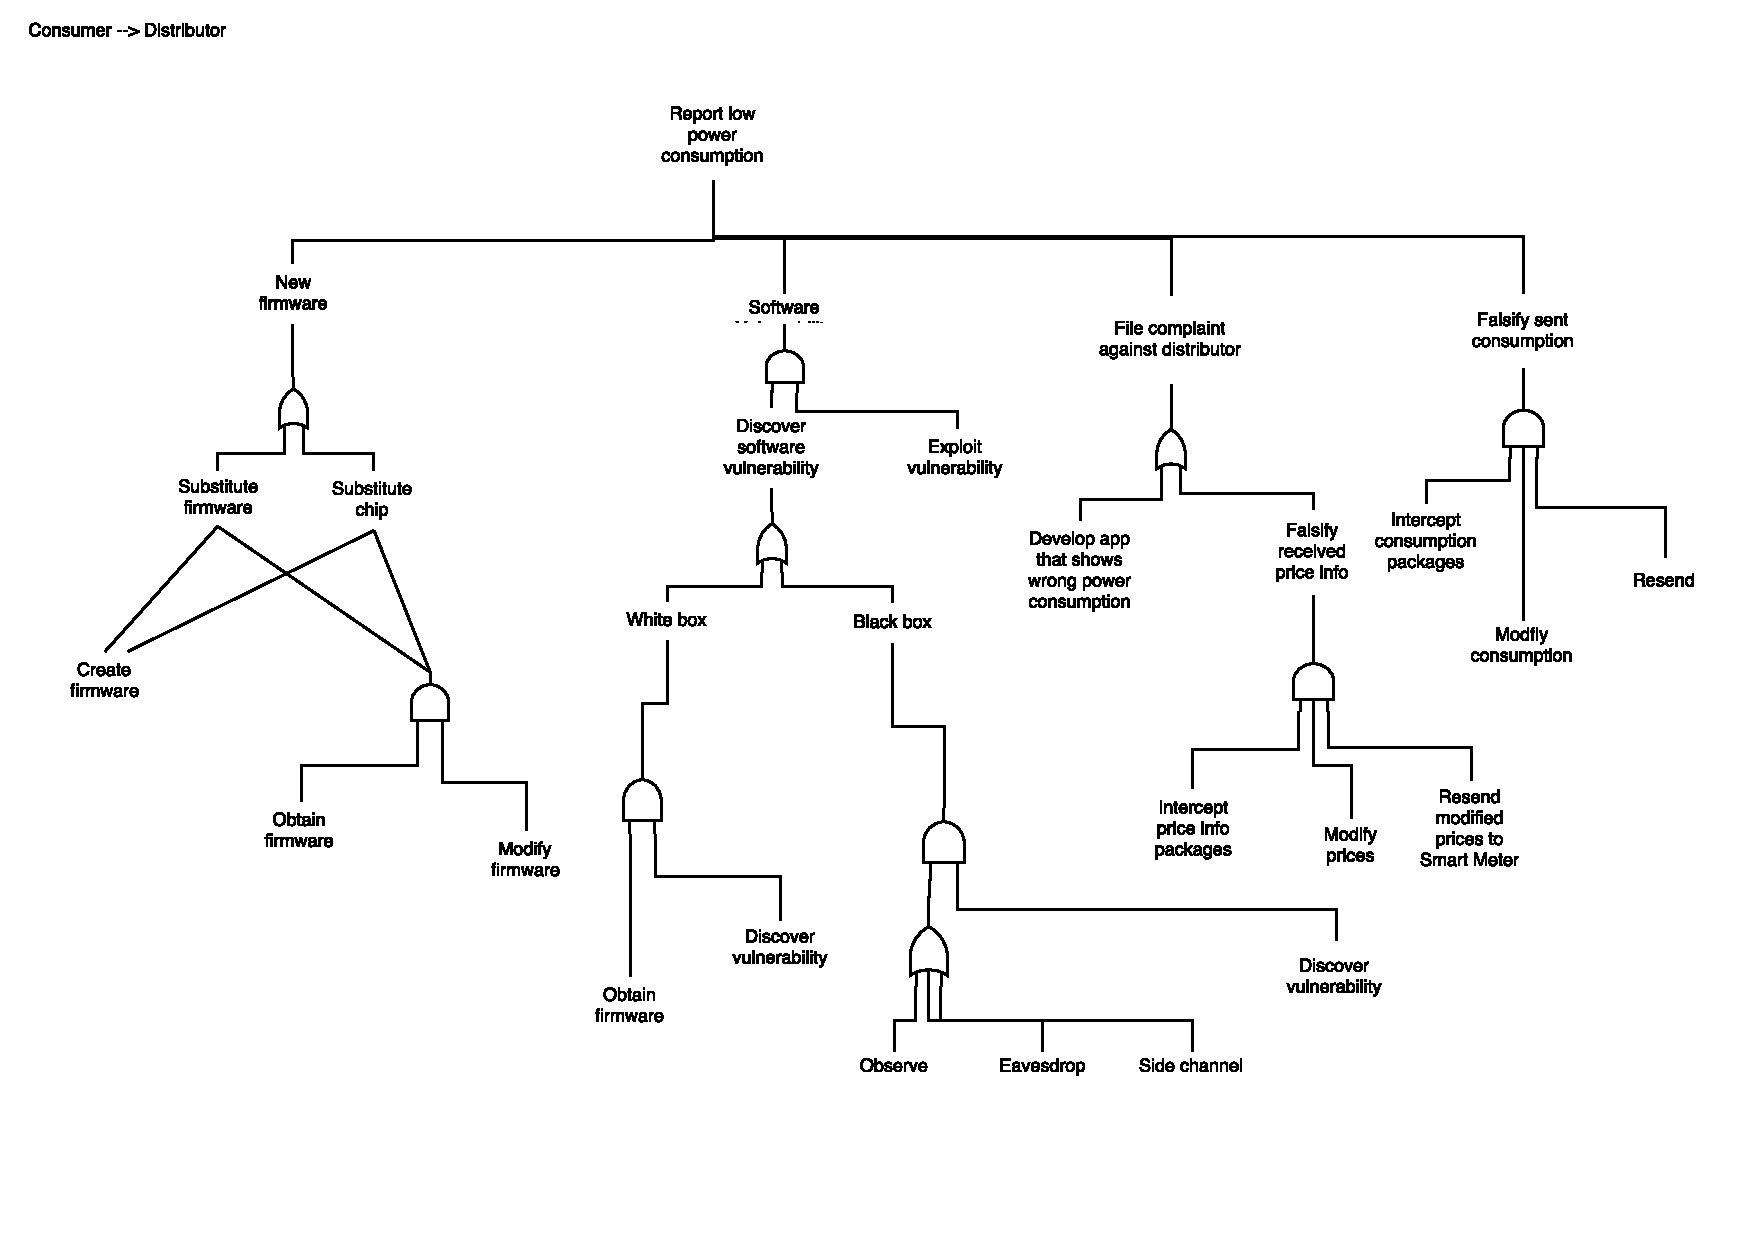
\includegraphics[width=\textheight, angle=90]{repport_low_power_consumtption_attack_tree.pdf}
  \caption{An attack tree where the costumer tries to report a low power consumption.}
  \label{report_power_attack_tree}
\end{figure}

\paragraph{Definition of an attack tree}
Attack trees consist of a set of nodes representing steps in a possible attack.
Inner nodes are represented as logic gates such that they do not represent a possible attack themselves but rather a rule describing how their children should be aggregated.
Thus a node represented by an AND gate would require all its child-nodes to be carried out successfully for it to be carried out successfully.

Additionally it should be noted that the attack tree is technically not a tree as it allows for the reuse of subnodes.
This is done to illustrate how certain steps can be part of multiple attacks.
We will however continue to use the term \emph{``attack trees''} to describe these structures.
\mikkel{\#8: Possibly insert litterature citation}

\subsection{Reporting a low power consumption}
To facilitate the reader in understanding the details of the attack tree in \cref{report_power_attack_tree} its nodes and sub-\emph{``trees''} will be described below.
In order for an electrical company to bill the consumer, he must first receive information from the smart meter about the consumers power consumption.
The root node splits the tree into four different possible attacks that all achieve this goal.
Each of these attacks will be described below.

\subsubsection{New firmware}
On the smart meter will be some firmware communicating with the meter's various electrical components.
This firmware will be running on one (or possibly several) microcontrollers.
Part of the firmware's responsibility is to report consumption to external entities as measured by the meter.

This attack describes the consumer replacing the firmware executed on the meter, either by uploading new firmware to the existing microcontroller(s) or by replacing the psysical controller(s).
The process of developing firmware will require the attacker to do either of the following;
\begin{itemize}
  \item \emph{Start from scratch}, building firmware based on the schematics of the smart meter.
  This process might require a great deal of trial-and-error if the attacker has litte knowledge of the smart meters instruction set.
  Some of this information might be obtained by eavesdropping on the running smart meter.
  \item Obtain a version of the existing firmware\footnote{Either as machine instructions or as some higher-level language.}.
    This firmware could then be modified as required by the attacker.
    But cryptography in the firmware could cause problems because even if modification of the firmware is possible keys used for communication will not be revealed.
\end{itemize}

\subsection{Software}
This process describes the same overall idea as the previous one.
It deals with knowledge about how the smart meter operates.
But instead of actually replacing the firmware the attacker will instead look for vulnerabilities in the implementation and exploit these.

This could be done by either by obtaining the smart meter's firmware as described above (white box) or by externally identifying key points in the smart meter processing (black box).
The details of this type of attack depends on the type of vulnerability found and will thus not be described further.

\subsubsection{Falsify sent comsumption}
Instead of attacking the smart meter itself, the attacker could choose to focus on its communication.
As the attacker (the consumer) is interested in what is reported to his power supplier, he could falsify this information instead.

He would intercept the packages sent from the meter, modify them and then resend them.
This approach will either require the data to be unencrypted, which does seem unlikely, or that the attacker has enough information about the system to decrypt and re-encrypt the packages.

Alternatively the attacker might intercept packages at times where he knows his power consumption to be low and resend them at a later point in time where he knows them to be high.

\subsubsection{File complaint}
As an alternative to the more technical approaches of the attacker we also propose another type of attack.
This involves the attacker attempting to prove that the power supplier are billing him for a too large power consumption.
This despite the bill actually corresponding with correct usage and price information.

The project group suggest two different approaches to achieving this goal:
\begin{enumerate}
  \item The user develops an application that mimics an official app describing the power consumption.
  This application will display an incorrectly low information about the consumers power consumption.
  \item The user successfully alters pricing information as received from the power supplier.
  He will want to lower the price locally, such that when he examines his ``expected bill'' the total price will be lower than that billed by the power supplier.
\end{enumerate}
Both of the above require the user to claim wrong-doing on behalf of the power supplier.
Any one individual might have a problem in assuring the validity of their claim.
However applying this attack on a larger scale will provide a possibly stronger case.

Additionally this type of attack might be carried out by the attacker on other consumers' smart meters, effectively hiding his intent by having multiple unaware consumers complain as well.
